\documentclass{article}
\title{Janim Example 3}
\author{John Doe}
\usepackage{tikz}
\usepackage{geometry}
\geometry{
paperheight=384mm,paperwidth=432mm,
total={344mm,392mm},
left=30mm,
top=30mm,
}
\usepackage{fontspec}
\usepackage{xcolor}
\setmainfont{CascadiaMono.ttf}
\pagenumbering{gobble}
\pagecolor{navy}
\hyphenpenalty 10000
\exhyphenpenalty 10000
\begin{document}
\maketitle
\noindent \textcolor{black}
{\Huge \textcolor{cyan}{Advanced \textcolor{magenta}{Layout} \textcolor{yellow}{and} \textcolor{green}{Styling}}}
\noindent \textcolor{black}
{\vspace{5mm}}

\begin{tikzpicture}
\filldraw[color=cyan!80, fill=transparent!0, very thick](15mm,15mm) circle (5mm);
\end{tikzpicture}

\begin{tikzpicture}
\filldraw[color=magenta!80, fill=transparent!0, very thick](15mm,402mm) circle (5mm);
\end{tikzpicture}

\begin{tikzpicture}
\filldraw[color=yellow!80, fill=transparent!0, very thick](354mm,15mm) circle (5mm);
\end{tikzpicture}

\begin{tikzpicture}
\filldraw[color=lime!80, fill=transparent!0, very thick](354mm,402mm) circle (5mm);
\end{tikzpicture}

\begin{tikzpicture}
\filldraw[color=cyan!60, fill=black!20, very thick](10mm,10mm) -- (10mm+8mm,10mm) -- (10mm+8mm/2,10mm+8mm) -- cycle;
\end{tikzpicture}

\begin{tikzpicture}
\filldraw[color=cyan!60, fill=black!20, very thick](10mm,407mm) -- (10mm+8mm,407mm) -- (10mm+8mm/2,407mm+8mm) -- cycle;
\end{tikzpicture}

\begin{tikzpicture}
\filldraw[color=cyan!60, fill=black!20, very thick](55mm,10mm) -- (55mm+8mm,10mm) -- (55mm+8mm/2,10mm+8mm) -- cycle;
\end{tikzpicture}

\begin{tikzpicture}
\filldraw[color=cyan!60, fill=black!20, very thick](55mm,407mm) -- (55mm+8mm,407mm) -- (55mm+8mm/2,407mm+8mm) -- cycle;
\end{tikzpicture}

\begin{tikzpicture}
\filldraw[color=cyan!60, fill=black!20, very thick](100mm,10mm) -- (100mm+8mm,10mm) -- (100mm+8mm/2,10mm+8mm) -- cycle;
\end{tikzpicture}

\begin{tikzpicture}
\filldraw[color=cyan!60, fill=black!20, very thick](100mm,407mm) -- (100mm+8mm,407mm) -- (100mm+8mm/2,407mm+8mm) -- cycle;
\end{tikzpicture}

\begin{tikzpicture}
\filldraw[color=cyan!60, fill=black!20, very thick](145mm,10mm) -- (145mm+8mm,10mm) -- (145mm+8mm/2,10mm+8mm) -- cycle;
\end{tikzpicture}

\begin{tikzpicture}
\filldraw[color=cyan!60, fill=black!20, very thick](145mm,407mm) -- (145mm+8mm,407mm) -- (145mm+8mm/2,407mm+8mm) -- cycle;
\end{tikzpicture}

\begin{tikzpicture}
\filldraw[color=cyan!60, fill=black!20, very thick](190mm,10mm) -- (190mm+8mm,10mm) -- (190mm+8mm/2,10mm+8mm) -- cycle;
\end{tikzpicture}

\begin{tikzpicture}
\filldraw[color=cyan!60, fill=black!20, very thick](190mm,407mm) -- (190mm+8mm,407mm) -- (190mm+8mm/2,407mm+8mm) -- cycle;
\end{tikzpicture}

\begin{tikzpicture}
\filldraw[color=cyan!60, fill=black!20, very thick](235mm,10mm) -- (235mm+8mm,10mm) -- (235mm+8mm/2,10mm+8mm) -- cycle;
\end{tikzpicture}

\begin{tikzpicture}
\filldraw[color=cyan!60, fill=black!20, very thick](235mm,407mm) -- (235mm+8mm,407mm) -- (235mm+8mm/2,407mm+8mm) -- cycle;
\end{tikzpicture}

\begin{tikzpicture}
\filldraw[color=cyan!60, fill=black!20, very thick](280mm,10mm) -- (280mm+8mm,10mm) -- (280mm+8mm/2,10mm+8mm) -- cycle;
\end{tikzpicture}

\begin{tikzpicture}
\filldraw[color=cyan!60, fill=black!20, very thick](280mm,407mm) -- (280mm+8mm,407mm) -- (280mm+8mm/2,407mm+8mm) -- cycle;
\end{tikzpicture}

\begin{tikzpicture}
\filldraw[color=cyan!60, fill=black!20, very thick](325mm,10mm) -- (325mm+8mm,10mm) -- (325mm+8mm/2,10mm+8mm) -- cycle;
\end{tikzpicture}

\begin{tikzpicture}
\filldraw[color=cyan!60, fill=black!20, very thick](325mm,407mm) -- (325mm+8mm,407mm) -- (325mm+8mm/2,407mm+8mm) -- cycle;
\end{tikzpicture}

\begin{tikzpicture}
\filldraw[color=magenta!60, fill=black!20, very thick](10mm,30mm) rectangle (10mm+6mm,30mm+6mm);
\end{tikzpicture}

\begin{tikzpicture}
\filldraw[color=magenta!60, fill=black!20, very thick](359mm,30mm) rectangle (359mm+6mm,30mm+6mm);
\end{tikzpicture}

\begin{tikzpicture}
\filldraw[color=magenta!60, fill=black!20, very thick](10mm,75mm) rectangle (10mm+6mm,75mm+6mm);
\end{tikzpicture}

\begin{tikzpicture}
\filldraw[color=magenta!60, fill=black!20, very thick](359mm,75mm) rectangle (359mm+6mm,75mm+6mm);
\end{tikzpicture}

\begin{tikzpicture}
\filldraw[color=magenta!60, fill=black!20, very thick](10mm,120mm) rectangle (10mm+6mm,120mm+6mm);
\end{tikzpicture}

\begin{tikzpicture}
\filldraw[color=magenta!60, fill=black!20, very thick](359mm,120mm) rectangle (359mm+6mm,120mm+6mm);
\end{tikzpicture}

\begin{tikzpicture}
\filldraw[color=magenta!60, fill=black!20, very thick](10mm,165mm) rectangle (10mm+6mm,165mm+6mm);
\end{tikzpicture}

\begin{tikzpicture}
\filldraw[color=magenta!60, fill=black!20, very thick](359mm,165mm) rectangle (359mm+6mm,165mm+6mm);
\end{tikzpicture}

\begin{tikzpicture}
\filldraw[color=magenta!60, fill=black!20, very thick](10mm,210mm) rectangle (10mm+6mm,210mm+6mm);
\end{tikzpicture}

\begin{tikzpicture}
\filldraw[color=magenta!60, fill=black!20, very thick](359mm,210mm) rectangle (359mm+6mm,210mm+6mm);
\end{tikzpicture}

\begin{tikzpicture}
\filldraw[color=magenta!60, fill=black!20, very thick](10mm,255mm) rectangle (10mm+6mm,255mm+6mm);
\end{tikzpicture}

\begin{tikzpicture}
\filldraw[color=magenta!60, fill=black!20, very thick](359mm,255mm) rectangle (359mm+6mm,255mm+6mm);
\end{tikzpicture}

\begin{tikzpicture}
\filldraw[color=magenta!60, fill=black!20, very thick](10mm,300mm) rectangle (10mm+6mm,300mm+6mm);
\end{tikzpicture}

\begin{tikzpicture}
\filldraw[color=magenta!60, fill=black!20, very thick](359mm,300mm) rectangle (359mm+6mm,300mm+6mm);
\end{tikzpicture}

\begin{tikzpicture}
\filldraw[color=magenta!60, fill=black!20, very thick](10mm,345mm) rectangle (10mm+6mm,345mm+6mm);
\end{tikzpicture}

\begin{tikzpicture}
\filldraw[color=magenta!60, fill=black!20, very thick](359mm,345mm) rectangle (359mm+6mm,345mm+6mm);
\end{tikzpicture}
\noindent \textcolor{black}
{\vspace{10mm}}
\noindent \textcolor{black}
{\textbf{\textcolor{white}{Color Palette Demonstration}}}
\noindent \textcolor{black}
{\vspace{3mm}}
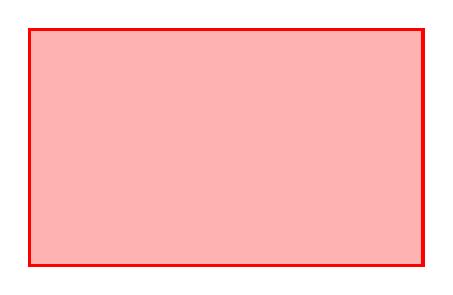
\begin{tikzpicture}
\filldraw[color=red!100, fill=red!30, very thick](30mm,60mm) rectangle (30mm+50mm,60mm+30mm);
\end{tikzpicture}
\noindent \textcolor{black}
{\textcolor{white}{\small \hspace{30mm}\vspace{-70mm}red}}

\begin{tikzpicture}
\filldraw[color=green!100, fill=green!30, very thick](90mm,60mm) rectangle (90mm+50mm,60mm+30mm);
\end{tikzpicture}
\noindent \textcolor{black}
{\textcolor{white}{\small \hspace{90mm}\vspace{-70mm}green}}
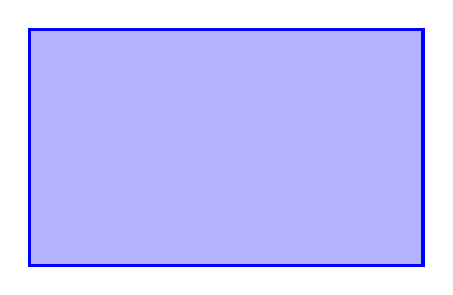
\begin{tikzpicture}
\filldraw[color=blue!100, fill=blue!30, very thick](150mm,60mm) rectangle (150mm+50mm,60mm+30mm);
\end{tikzpicture}
\noindent \textcolor{black}
{\textcolor{white}{\small \hspace{150mm}\vspace{-70mm}blue}}

\begin{tikzpicture}
\filldraw[color=cyan!100, fill=cyan!30, very thick](210mm,60mm) rectangle (210mm+50mm,60mm+30mm);
\end{tikzpicture}
\noindent \textcolor{black}
{\textcolor{white}{\small \hspace{210mm}\vspace{-70mm}cyan}}
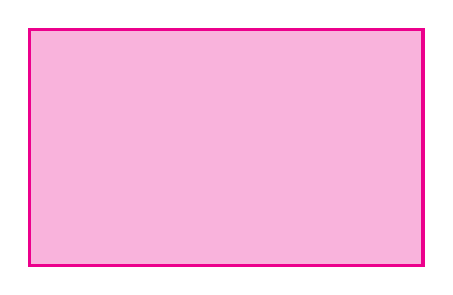
\begin{tikzpicture}
\filldraw[color=magenta!100, fill=magenta!30, very thick](270mm,60mm) rectangle (270mm+50mm,60mm+30mm);
\end{tikzpicture}
\noindent \textcolor{black}
{\textcolor{white}{\small \hspace{270mm}\vspace{-70mm}magenta}}

\begin{tikzpicture}
\filldraw[color=yellow!100, fill=yellow!30, very thick](30mm,100mm) rectangle (30mm+50mm,100mm+30mm);
\end{tikzpicture}
\noindent \textcolor{black}
{\textcolor{white}{\small \hspace{30mm}\vspace{-110mm}yellow}}

\begin{tikzpicture}
\filldraw[color=orange!100, fill=orange!30, very thick](90mm,100mm) rectangle (90mm+50mm,100mm+30mm);
\end{tikzpicture}
\noindent \textcolor{black}
{\textcolor{white}{\small \hspace{90mm}\vspace{-110mm}orange}}

\begin{tikzpicture}
\filldraw[color=purple!100, fill=purple!30, very thick](150mm,100mm) rectangle (150mm+50mm,100mm+30mm);
\end{tikzpicture}
\noindent \textcolor{black}
{\textcolor{white}{\small \hspace{150mm}\vspace{-110mm}purple}}

\begin{tikzpicture}
\filldraw[color=pink!100, fill=pink!30, very thick](210mm,100mm) rectangle (210mm+50mm,100mm+30mm);
\end{tikzpicture}
\noindent \textcolor{black}
{\textcolor{white}{\small \hspace{210mm}\vspace{-110mm}pink}}

\begin{tikzpicture}
\filldraw[color=lime!100, fill=lime!30, very thick](270mm,100mm) rectangle (270mm+50mm,100mm+30mm);
\end{tikzpicture}
\noindent \textcolor{black}
{\textcolor{white}{\small \hspace{270mm}\vspace{-110mm}lime}}
\noindent \textcolor{black}
{\vspace{60mm}}
\noindent \textcolor{black}
{\textbf{\textcolor{white}{Overlapping Shapes Pattern}}}
\noindent \textcolor{black}
{\vspace{3mm}}
\begin{tikzpicture}
\filldraw[color=red!80, fill=transparent!0, very thick](200mm,250mm) circle (40mm);
\end{tikzpicture}
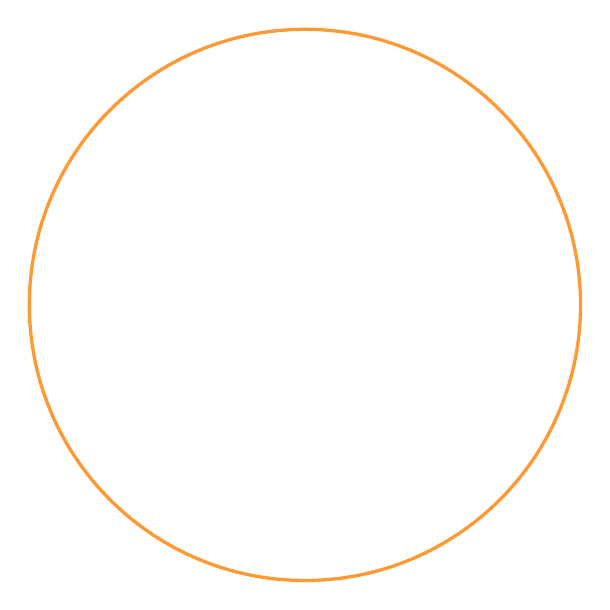
\begin{tikzpicture}
\filldraw[color=orange!80, fill=transparent!0, very thick](200mm,250mm) circle (35mm);
\end{tikzpicture}
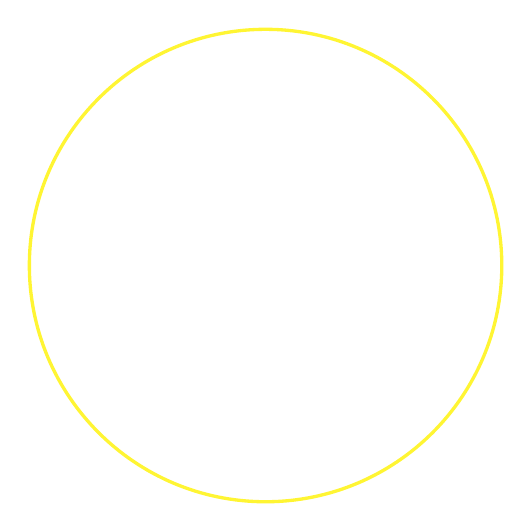
\begin{tikzpicture}
\filldraw[color=yellow!80, fill=transparent!0, very thick](200mm,250mm) circle (30mm);
\end{tikzpicture}
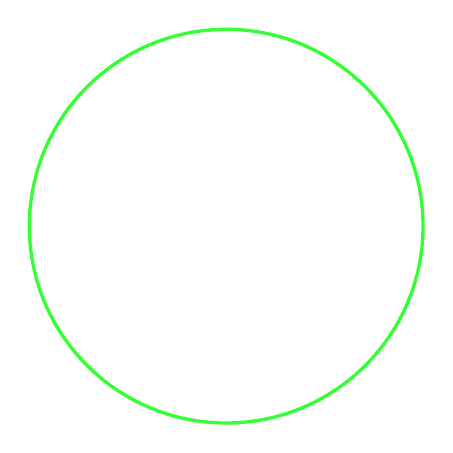
\begin{tikzpicture}
\filldraw[color=green!80, fill=transparent!0, very thick](200mm,250mm) circle (25mm);
\end{tikzpicture}
\begin{tikzpicture}
\filldraw[color=blue!80, fill=transparent!0, very thick](200mm,250mm) circle (20mm);
\end{tikzpicture}
\begin{tikzpicture}
\filldraw[color=indigo!80, fill=transparent!0, very thick](200mm,250mm) circle (15mm);
\end{tikzpicture}
\begin{tikzpicture}
\filldraw[color=violet!80, fill=transparent!0, very thick](200mm,250mm) circle (10mm);
\end{tikzpicture}
\begin{tikzpicture}
\draw[color=white, thin] (160mm,210mm)--(240mm,290mm);
\end{tikzpicture}
\begin{tikzpicture}
\draw[color=white, thin] (240mm,210mm)--(160mm,290mm);
\end{tikzpicture}
\begin{tikzpicture}
\draw[color=white, thin] (160mm,250mm)--(240mm,250mm);
\end{tikzpicture}
\begin{tikzpicture}
\draw[color=white, thin] (200mm,210mm)--(200mm,290mm);
\end{tikzpicture}
\noindent \textcolor{black}
{\vspace{80mm}}
\noindent \textcolor{black}
{\textcolor{white}{This document demonstrates advanced features of Janim:}}
\noindent \textcolor{black}
{\begin{itemize}}
\noindent \textcolor{black}
{\item Custom page styling with navy background and colored elements}
\noindent \textcolor{black}
{\item Decorative borders and corner ornaments}
\noindent \textcolor{black}
{\item Color palette visualization}
\noindent \textcolor{black}
{\item Overlapping shapes and patterns}
\noindent \textcolor{black}
{\item Precise positioning of elements}
\noindent \textcolor{black}
{\end{itemize}}
\end{document}
